\subsection{Nabomatricer}
En anden mulighed for at repræsentere en graf er ved brug af \emph{nabomatricer}. Nabomatricer er bedre, når grafen har mange kanter, da man her kan se hvor mange kanter et givent knudepar har.
En nabomatrix kan beskrives som en $N=m \times m$-matrix, hvor $m$ er afhængig af knudemængden $V=\{v_1, v_2, \dotsc, v_m\}$. Hvis man har en simpel graf, $G=(V,E)$, vil matricen være en 0-1-matrix, da en simpel graf kun kan have en kant mellem to knuder. Når der er en kant mellem to  vilkårlig knuder, $a_{ij}=(v_i,v_j)$,  vil den få notationen 1, hvis der derimod ikke er en kant, får den notationen 0.
Det kan også skrives som
\begin{equation}
	a_{ij} =	
	\begin{cases}
		1 \mbox{ hvis } (v_i,v_j) \\
		0 \mbox{ ellers }.
	\end{cases}
\end{equation}

\begin{figure}[H]
  \centering
  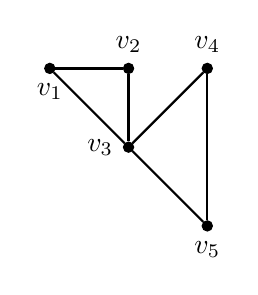
\begin{tikzpicture}
  \tikzset{enclosed/.style={draw, circle, inner sep=0pt, minimum size=.13cm, fill=black}}
  	\node[enclosed] at (0,2) (v1) [label=below:\(v_1\)] {};
    \node[enclosed] at (1,2) (v2) [label=above:\(v_2\)] {};
    \node[enclosed] at (1,1) (v3) [label=left:\(v_3\)] {};
    \node[enclosed] at (2,2) (v4) [label=above:\(v_4\)] {};
    \node[enclosed] at (2,0) (v5) [label=below:\(v_5\)] {};
    
	\path[thick] (v1) edge node {} (v2);
	\path[thick] (v1) edge node {} (v3);
	\path[thick] (v2) edge node {} (v3);
	\path[thick] (v4) edge node {} (v3);
	\path[thick] (v5) edge node {} (v3);   
	\path[thick] (v4) edge node {} (v5); 

  \end{tikzpicture}
  \caption{Ikke-orienteret, simpel graf til matrix.}
  \label{fig:stm}
\end{figure}

Vi opstiller nabomatricen for \autoref{fig:stm} således:
\begin{equation} \label{mat:nabo1}
\begin{blockarray}{rccccc}
		&v_1&v_2&v_3&v_4&v_5 \\
\begin{block}{r[ccccc]}
		v_1&0&1&1&0&0 \\
		v_2&1&0&1&0&0 \\
		v_3&1&1&0&1&1 \\
		v_4&0&0&1&0&1 \\
		v_5&0&0&1&1&0 \\
\end{block}
\end{blockarray}
\end{equation}

Nabomatricen for \autoref{fig:ikke-orienteret-pseudo}, som har multiple kanter mellem to knuder, vil se ud således.

\begin{equation}
\begin{blockarray}{rccccccc}
	&v_1&v_2&v_3&v_4&v_5&v_6&v_7 \\
\begin{block}{r[ccccccc]}
	v_1&0&1&1&0&0&0&0 \\
	v_2&1&0&1&0&0&0&0 \\
	v_3&1&1&0&2&1&0&0 \\
	v_4&0&0&2&0&1&1&1 \\
	v_5&0&0&1&1&0&1&0 \\
	v_6&0&0&0&1&1&0&1 \\
	v_7&0&0&0&1&0&1&1 \\
\end{block}
\end{blockarray}	
\end{equation}

Det kan ses, at der er 2 kanter, der er incidente med knudeparret $v_3$ og $v_4$. Derudover kan det ses, at der er en løkke ved $v_7$.

